\chapter{РЕАЛИЗАЦИЯ СИСТЕМЫ УПРАВЛЕНИЯ ДВИЖЕНИЕМ БЕСПИЛОТНОГО АВТОМОБИЛЯ}
В этой главе рассматривается реализация системы управления движением беспилотного автомобиля на основе разработанного
в предыдущей главе алгоритма, а также создание модели автомобиля для тестирования и отработки системы.

\section{Использование ROS в качестве основы для системы управления}
Разработка комплексного программного обеспечения, которым является система управления беспилотным автомобилем ~---
сложная и объемная задача. Система управления состоит из ряда модулей, которые должны взаимодействовать друг с другом.
Также требуется обеспечить работу с внешними устройствами, такими как стереокамера и LiDAR. Система управления должна
состоять из следующих модулей:
\begin{itemize}
    \item модуль получения видео со стереокамеры,
    \item модуль получения облака точек с LiDAR,
    \item модуль, реализующий алгоритм SLAM для определения положения и ориентации автомобиля в пространстве с помощью
          стероекамеры,
    \item модуль планирования движения,
    \item модуль движения по программной траектории,
    \item модуль управления двигателями,
    \item модуль пользовательского интерфейса для управления, визуализации и отладки системы.
\end{itemize}

Как видно, система состоит из большого числа модулей, для части из которых (работа с камерой и LiDAR, алгоритм SLAM)
существуют готовые реализации. Необходимо реализовать модули достаточно независимыми, чтобы обеспечить легкость тестирования
и возможность дальнейшего расширения и модернизации системы, что требует реализации способа взаимодействия между модулями.

Эта проблема широко распространена в сфере робототехники, и существует ряд решений, облегчающих разработку. Одним из
таких решений является Robot Operation System (ROS) \cite{ros}.

Robot Operating System ~--- это гибкий фреймворк для написания программного обеспечения для роботов. Он включает в себя
набор инструментов, библиотек и соглашений, направленных на упрощение создания сложных систем управления для широкого
класса робототехнических платформ. ROS является одним из самых широко распространенных фреймворком для разработки
программного обеспечения для робототехнических систем.

Использование ROS обладает рядом преимуществ, таких как:
\begin{itemize}
    \item поддерживает модульную и распределенную архитектуру приложений;
    \item обладает готовыми удобными механизмами взаимодействия между модулями;
    \item имеет большое количество утилит и инструментов, таких как программы с графическим интерфейсом, для отображения
          множества данных (изображения, облака точек, траектории и т.д.), логгер, позволяющий записывать данные,
          передаваемые между модулями, и потом воспроизводить их для дальнейшего изучения и отладки, визуализатор
          модулей, из которых состоит система, система сборки, облегчающая компиляцию и многое другое;
    \item множество готовых библиотек для управления, компьютерного зрения и визуализации;
    \item подробная документация;
    \item обширное сообщество разработчиков.
\end{itemize}

В основе ROS лежит концепция узла или ноды (node). Нода ~--- это базовая единица построения ПО в ROS, программный модуль,
который выполняет определенное действие, например, работает с LiDAR и предоставляет облака точек, и представляет
собой отдельный процесс. Ноды взаимодействуют с помощью IPC (inter-process communication) механизмов, предоставляемых
ROS: топиков (ROS topic) и сервисов (ROS service). Ноды ROS могут быть реализованы на различных языках программирования.
Официально поддерживаются C++, Python 2.7 и Common Lisp, для этих языков реализованы клиентские библиотеки, позволяющие
получить доступ к возможностям ROS. Существуют клиентские библиотеки для других языков, таикх как C\#, Java, JavaScript,
Ruby, Lua, Go, но большинство из них не обновляются и не поддерживают современные версии ROS. Помимо этого, существует
пакет ROS "rosbridge\_suite", предоставляющий интерфейс ROS в виде JSON-API, что позволяет использовать ROS с любым языком,
в котором можно работать с сетью и JSON.

Топики реализуют механизм "издатель-подписчик". Топик является именованной типизированной FIFO очередью, в которую
ноды могут асинхронно записывать данные и считывать данные. Ноды, которые записывают данные в топик называются
издатель (publisher), а ноды, которые считывают данные из ноды, называются подписчик (subscriber). Несколько нод могут
одновременно писать и читать данные из одного топика.

Данные представляются в виде сообщений (messages). Сообщение
представляет собой структуру данных, которая может состоять из примитивных типов данных, таких как целые числа или
строки, и других типов данных, например, основанных на других сообщениях. Для описание сообщений в ROS применяются
файлы специального формата, в которых перечисляются все тип и название всех полей сообщения. На основе этих файлов
сборочная система ROS осуществляет генерацию кода для представления сообщения в поддерживаемых языках программирования.
Так, например, для C++ и Python создаются классы с соответствующими полями и внутренний вспомогательный код для сериализации
сообщений. ROS имеет большое количество встроенныхс стандартных типов сообщений, типичных для робототехники, такие как
изображение (sensors\_msgs/Image), облака точек (sensors\_msgs/PointCloud2), положение и кватернион ориентации
(geometry\_msgs/Pose), путь, как набор положений (nav\_msgs/Path), карта препятствий в виде сетки (nav\_msgs/OccupancyGrid)
и многие другие.

Преимуществом такого механизма является то, что отдельные ноды могут быть полностью независимы от других и не иметь
никакой информации о них. Например, для ноды, занимающающейся обработкой облака точек, совершенно не важно, получены
ли данные от LiDAR, камеры глубины, такой как Kinect, от стереокамеры или даже воспроизводятся из файла ~---
данные приходят в одинаковом стандартном формате.

Другим способом взаимодействия между нодами в ROS являются сервисы, реализующие механизм "запрос-ответ". В данном случае
одна нода выступает в роле сервиса, а другие ~--- в роли клиентов. Сервисы, в отличие, от топиков, являются синхронными,
т.е. нода, обратившаяся к сервису, ожидает ответа от него. Для описания сервисов также существует определенный формат
файла, в котором описываются типы и имена агументов, передаваемые клиентом сервису, и формат ответа от сервиса.
Таким образом, сервис реализует семантику удаленного вызова процедуры (Remote Procedure Call).

ROS обладает центральным узлом ~--- мастером (ROS Master), который отвечает за соединение между собой всех узлов ROS.
Мастер хранит информацию обо всех подписках, публикациях, сервисах и предоставляет эту информацию нодам. Взаимодействие
между нодами и мастером осуществляется по протоколу XML/RPC, дальнейшее взаимодействие нод между собой может осуществляться
по ряду протоколов, чаще всего применяется TCP.

На рисукне \ref{img:ros_topic_mechainism} приведена иллюстрация механизма установления соединения между двумя нодами
при использовании топиков.

\begin{figure}[h]
    \centering
    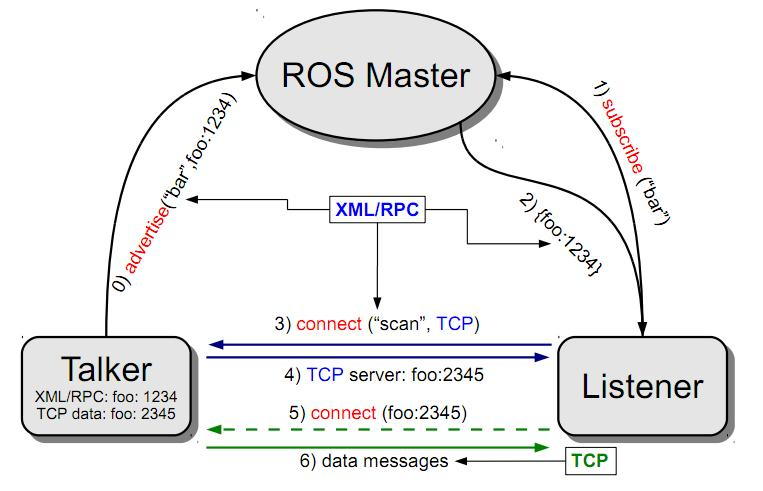
\includegraphics[width=\linewidth]{images/3_devel/ros_topic}
    \caption{Механизм работы топиков ROS}
    \label{img:ros_topic_mechainism}
\end{figure}

Нода, выступающая в роле издателя уведомляет об этом мастера, вызывая метод "advertise" с использованием протокола XML/RPC,
сообщая ему имя топика и тип сообщения. Нода, выступающая в качестве подписчика, отправляет запрос "subscribe" мастеру
с использованием протокола XML/RPC, сообщая имя топика, на который осуществляется подписка. В ответ мастер сообщает
данные для подключения к ноде-издателю. После этого нода-слушатель отправляет запрос "connect" ноде-издателю с
использованием протокола XML/RPC. В ответ нода-издатель сообщает данные (адрес и порт) для установления TCP-соединения.
После этого нода-подписчик осуществляет TCP-подключение к ноде-издателю и после этого нода-издатель может осуществлять
передачу данных.

Механизм работы сервисов приведен на рисунке \ref{img:ros_service_mechainism}.

\begin{figure}[h]
    \centering
    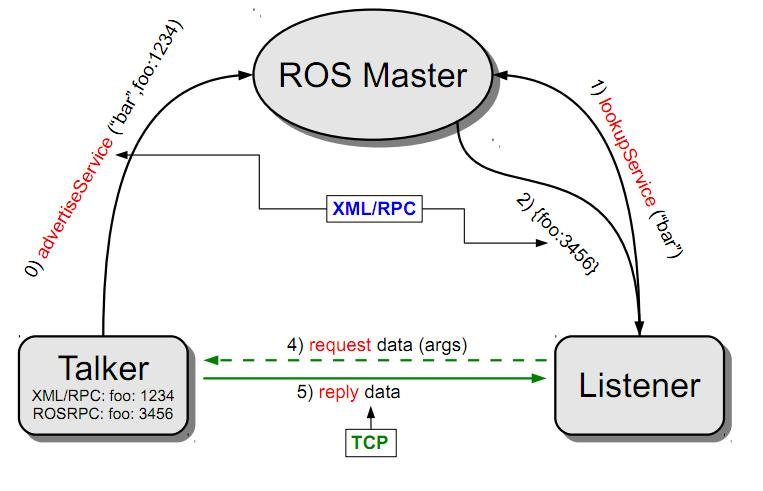
\includegraphics[width=\linewidth]{images/3_devel/ros_service}
    \caption{Механизм работы топиков ROS}
    \label{img:ros_service_mechainism}
\end{figure}

В данном случае нода, выступающая в роли сервиса, уведомляет об этом мастера, вызывая метод "advertiseService" с
использованием протокола XML/RPC. Нода, использующая сервис, вначале запрашивает у мастера данные для вызова сервиса,
вызывая метод "lookupService" с использованием протокола XML/RPC. Мастер сообщает данные  для подключения (адрес и порт).
После этого, когда требуется вызвать сервис, нода устанавливает TCP-подключение, отправляет запрос и принимает ответ
от ноды-сервиса.

Существует два режима работы сервисов: с установлением соединения на каждый запрос (по-умолчанию), и с постоянным
соединением. Первый режим более надежен, т.к. позволит работать даже в случае перезапуска сервиса, а второй режим
обеспечивает меньшую латентность вызова сервиса. Результаты измерения латентности вызова сервиса в режиме повторного
подключения и режиме постоянного подключения в пределах localhost представлены на рисунке
\ref{img:rosservice_call_latency} и в таблице \ref{tab:rosservice_call_latency}. Из результатов измерения видно,
что постоянное подключение обеспечивает существенно меньшую латентность вызова и, что не менее важно, меньший
джиттер (разброс времени вызова), что особенно важно для систем реального времени.

\begin{figure}[h]
    \centering
    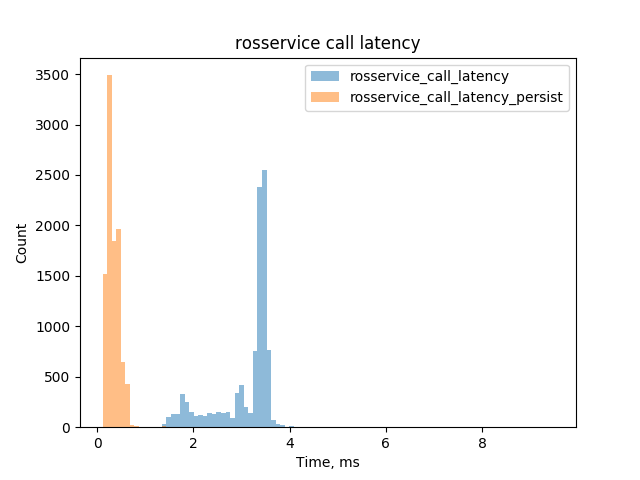
\includegraphics[]{images/3_devel/rosservice_call_latency}
    \caption{Механизм работы топиков ROS}
    \label{img:rosservice_call_latency}
\end{figure}

\begin{table}[h]
    \caption{Сравнение латентности вызова сервисов ROS в разных режимах}
    \label{tab:rosservice_call_latency}
    \begin{tabularx}{\textwidth}{|l|X|X|}
        \hline
                     & Повторное подключение, мс & Постоянное подключение, мс \\
        \hline
        Минимальное  & 1.2 & 0.1 \\
        \hline
        Среднее      & 3.1 & 0.4 \\
        \hline
        Максимальное & 9.5 & 1.1 \\
        \hline
    \end{tabularx}
\end{table}

\section{Постройка мобильной платформы}


\section{Реализация управления приводами мобильной платформы}
\section{Реализация подсистемы распознавание препятствий}
\section{Реализация подсистемы планирования траектории}
\section{Реализация подсистемы следования траектории}